\documentclass[10pt]{article}
\usepackage[margin=0.75in]{geometry}
\usepackage[T1]{fontenc}
\usepackage{amsmath,amssymb,booktabs,longtable,array,hyperref}
\usepackage{tikz}
\usetikzlibrary{arrows.meta,positioning}
\hypersetup{colorlinks=true,urlcolor=blue,linkcolor=blue}
\newcommand{\W}{W(3,3)}
\newcommand{\pf}[1]{\texttt{\detokenize{#1}}}
\title{\textbf{The Photonic Hardware Atlas}\\A Traceable Circuit, Control, and Measurement Blueprint for W33}
\author{W33-Theory engineering programme}
\date{23 October 2026 -- Initial schematic edition}
\begin{document}
\maketitle
\begin{abstract}
This living atlas connects W33 quantum-information targets to circuits, virtual controller channels, proposed optical components, experimental observables, and eventual foundry sign-off. Its first executable release eliminates a redundant 120-angle gauge in an existing 376-parameter, 16-mode Givens implementation. A JSON contract enumerates 120 two-mode cells, 16 input-side phase cells, 256 virtual logical control channels, and measurement families. These are software and mathematical results, not a routed chip, an operating quantum computer, a PDK-qualified design, or laboratory calibration.
\end{abstract}
\tableofcontents

\section{Scope and source provenance}
The primary theory source is \pf{papers/forty_points/main.pdf} (202 pages). Printed page 131 explicitly distinguishes machine specification from a built device. The root \pf{photonic_holonet.tex}, \pf{holonet_machine_blueprint.tex}, and included body files supply broader architecture. The 16-mode compiler lineage is \pf{analysis/w33_levi_next5_v2_photonic.py}, \pf{analysis/w33_levi_next5_v3_tolerance.py}, \pf{analysis/w33_levi_next5_v4_foundry.py}, and \pf{analysis/w33_levi_next5_v5_hybrid.py}. The existing \pf{hardware/README_v5.md} clearly identifies its GDS as an abstract placement sketch. October 21 arithmetic-Frobenius optical-surrogate work also shows that native nonunitary operators cannot automatically be implemented with passive unitary optics. All design and experiment claims here are tiered by provenance.

\begin{longtable}{p{0.25\linewidth}p{0.40\linewidth}p{0.25\linewidth}}
\toprule Status & Supported & Not supported\\\midrule
Exact / numeric & Halmos target, Givens decomposition, gauge identity and reconstruction & Loss and experimental phase response\\
Executable schematic & Logical optical nets, parameter names, virtual driver channels and unit tests & Lithographic geometry and pinout\\
Design proposal & PZT, Pockels and measurement architectures & Process-compatible devices or fabrication\\
Experimental proposal & Coherent amplitude and photon-counting protocol & Real calibration, detector data, fault-tolerance\\
Foundry-ready & None in this initial edition & DRC, LVS, PDK extraction, yield, packing\\\bottomrule
\end{longtable}

\section{Exact mathematics and the electrode-count trap}
For the source $8\times8$ matrix $A$, let $s$ be its largest singular value and $C=A/s$. The Halmos dilation is
\[
U_H=\begin{pmatrix}
C&(I-CC^\dagger)^{1/2}\\
(I-C^\dagger C)^{1/2}&-C^\dagger
\end{pmatrix}\in U(16).
\]
The upstream Gaussian elimination gives 120 SU(2) two-mode rotations and a diagonal with 16 phases. An individual rotation is
\[
G(\theta,\phi,\alpha)=
\begin{pmatrix}
e^{i\alpha}\cos\theta&e^{i(\alpha+\phi)}\sin\theta\\
-e^{-i(\alpha+\phi)}\sin\theta&e^{-i\alpha}\cos\theta
\end{pmatrix}
=D_\alpha R(\theta,\phi),
\]
where $D_\alpha=\operatorname{diag}(e^{i\alpha},e^{-i\alpha})$ and
\[
R(\theta,\phi)=\begin{pmatrix}
\cos\theta&e^{i\phi}\sin\theta\\
-e^{-i\phi}\sin\theta&\cos\theta
\end{pmatrix}.
\]
Since $P R^\dagger(\theta,\phi)=R^\dagger(\theta,\phi+\delta_i-\delta_j)P$ for diagonal $P$ carrying phases $\delta_i,\delta_j$, each $\alpha$ is moved to later gates and the terminal diagonal:
\[
\phi_k'=\phi_k+\delta_{i(k)}-\delta_{j(k)},\quad
\delta_{i(k)}\leftarrow\delta_{i(k)}-\alpha_k,\quad
\delta_{j(k)}\leftarrow\delta_{j(k)}+\alpha_k.
\]
Therefore the algebraic $120(3)+16=376$ coordinate description becomes $120(2)+16=256$ logical coordinates without changing the synthesized unitary. This agrees with $\dim_{\mathbb R}U(16)=256$. The local regression confirms gauge-equivalence to the original synthesized circuit within $10^{-11}$; the upstream target reconstruction residual remains approximately $5.44\cdot10^{-9}$ because of floating-point matrix square roots.

\subsection{The special real target}
The v5 target is numerically real orthogonal; after gauge reduction all $\phi_k$ and terminal diagonal phases are $0$ or $\pi$ modulo floating-point tolerance, while all 120 nominal mixing angles are nonzero. This suggests a \emph{specialized} real orthogonal mesh with 120 continuously tunable mixing angles and binary programmed phase states. It is not proof that only 120 fabricated phase elements suffice: trims, crosstalk compensation, drift, and physical MZI decomposition can increase the required actuator count. An actual electrode count demands process-specific ports and a measured Jacobian.

\subsection{Candidate balanced-coupler identity}
With $H=2^{-1/2}\left(\begin{smallmatrix}1&1\\1&-1\end{smallmatrix}\right)$ and $D(t)=\operatorname{diag}(e^{it},e^{-it})$,
\[
R^\dagger(\theta,\phi)=D(\gamma)HD(\theta)HD(-\gamma),
\qquad\gamma=\frac{\phi+\pi/2}{2}.
\]
This is an algebraic two-balanced-coupler construction. The conjugate boundary phases may require more than one physical phase-shifter section and may be shared with neighboring stages. No PDK-compatible device or electrode count is inferred.

\section{Logical optical circuit diagram and port map}
\begin{center}
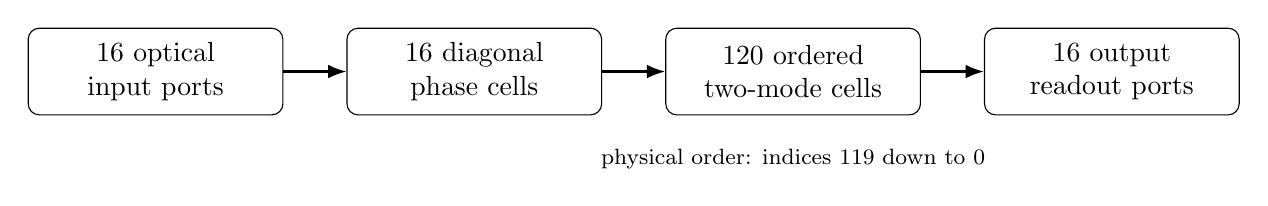
\begin{tikzpicture}[>=Latex,blk/.style={draw,rounded corners,align=center,text width=30mm,minimum height=11mm},node distance=8mm]
\node[blk] (a) {16 optical\\input ports};
\node[blk,right=of a] (b) {16 diagonal\\phase cells};
\node[blk,right=of b] (c) {120 ordered\\two-mode cells};
\node[blk,right=of c] (e) {16 output\\readout ports};
\draw[->,thick](a)--(b);\draw[->,thick](b)--(c);\draw[->,thick](c)--(e);
\node[below=3mm of c,font=\footnotesize,align=center] {physical order: indices 119 down to 0};
\end{tikzpicture}
\end{center}
Crucial ordering correction: in the compiler convention $U=G_0^\dagger\cdots G_{119}^\dagger D$, so the rightmost diagonal $D$ acts at the physical \emph{input}, although the original code calls it output phases following left-Givens elimination.

The emitted \pf{data/w33_photonic_control_netlist_20261023.json} contains the complete electrical/optical \emph{logical} map. Cell identifiers are MZI\_000 through MZI\_119, with two optical inputs, two optical outputs, and the pair of logical theta/phi controls. INPUT\_PHASE\_00 through INPUT\_PHASE\_15 precede the mesh. There are 256 distinct VIRTUAL\_DRV identifiers and 256 distinct control IDs. Optical rails are wired in physically applied (reverse algebraic) sequence; no port fan-out is implicitly invented.

\begin{center}
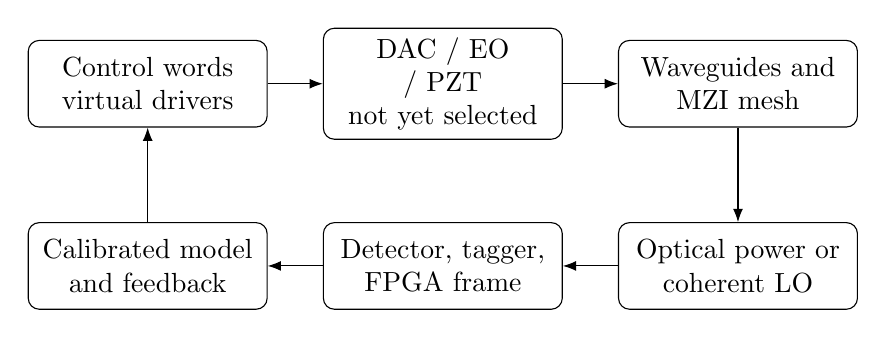
\begin{tikzpicture}[>=Latex,blk/.style={draw,rounded corners,align=center,text width=28mm,minimum height=11mm},node distance=7mm]
\node[blk] (driver) {Control words\\virtual drivers};
\node[blk,right=of driver] (eo) {DAC / EO / PZT\\not yet selected};
\node[blk,right=of eo] (light) {Waveguides and\\MZI mesh};
\node[blk,below=12mm of light] (det) {Optical power or\\coherent LO};
\node[blk,left=of det] (count) {Detector, tagger,\\FPGA frame};
\node[blk,left=of count] (servo) {Calibrated model\\and feedback};
\draw[->](driver)--(eo);\draw[->](eo)--(light);\draw[->](light)--(det);
\draw[->](det)--(count);\draw[->](count)--(servo);\draw[->](servo)--(driver);
\end{tikzpicture}
\end{center}
The existing v5 GDS contains 120 abstract rectangles in a separate nominal geometry. No validated one-to-one equivalence between these rectangles and the ordered Reck gates is claimed. A Clements lowering and routed physical implementation must each be independently reconstructed.

\section{Components and circuit-specific interfaces}
\begin{longtable}{p{0.23\linewidth}p{0.34\linewidth}p{0.32\linewidth}}
\toprule Component & Input/output or signal contract & Required validation\\\midrule
Photon source / herald & optical excitation, herald TTL, clock reference & spectrum, purity, loss and SPAM\\
Waveguide bus (16 rails) & 16 optical input and output ports & confinement, bends, crossings, propagation loss\\
Balanced coupler / splitter & two optical inputs and two outputs & splitting ratio and wavelength response\\
Programmable two-mode cell (120) & two optical ports per side; theta/phi targets & scattering matrix, netlist and actuators\\
Diagonal input phase (16) & one input optical rail, logical phase & absolute/relative reference and trim\\
PZT coarse actuator & electrical voltage or charge / piezo response & foundry compatibility, hysteresis, bandwidth\\
Pockels fine actuator & drive electrode pair / EO phase & $V_\pi$, capacitance, EO loss and RF bandwidth\\
Monitor and LO & coherent field or output power & phase stabilization and tap loss\\
Detector and tagger & pulse, channel, timestamp, overflow & jitter, dark count, dead time and efficiency\\
FPGA reducer & valid/ready streams, counts, timestamps & hardware-in-loop timing and clock crossing\\
Control estimator & commanded phases and measurement residuals & Jacobian conditioning and drift covariance\\
Packaging & optical fibers, electrical pads and grounds & parasitics, heat, ESD, assembly and test\\\bottomrule
\end{longtable}

\section{Measurements: what is observable and what is not}
For any input-side diagonal phase $D_{\mathrm{in}}$, basis-state power measurements obey
\[
|(U D_{\mathrm{in}})_{oi}|^2=|U_{oi}|^2.
\]
Thus 16 basis-injection settings and 16 power outputs per setting yield 256 real measurements, but cannot identify the rightmost input-phase bank. The executable certificate perturbs one input phase and checks invariant intensities alongside a changed complex transfer matrix. This is a precise observability obstruction, not a proof that every internal control is unobservable.

\begin{longtable}{p{0.25\linewidth}p{0.37\linewidth}p{0.27\linewidth}}
\toprule Measurement family & Proposed observable & Evidence boundary\\\midrule
BASIS\_00--15 & 16 output powers per one-mode input (256 real samples) & input phase gauge invisible\\
COHERENT\_00--15 & 16 complex transfer samples per input relative to stable LO & requires calibrated phase reference and SPAM\\
Small actuator perturbations & complex matrix derivatives; sensitivity Jacobian & physical Jacobian rank not yet measured\\
Thermal / EO drift & output drift, correlation and servo bandwidth & process-specific model not certified\\
Herald / coincidence & single-photon probability, loss, $g^{(2)}$, syndrome statistics & quantum experiments not performed\\\bottomrule
\end{longtable}
A transfer-function calibration with classical coherent light does not certify a universal quantum computer, entanglement, magic-state injection, or a fault-tolerance threshold. Detector response, source drift, coherent reference errors, and missing ports must be treated explicitly.

\section{Verification and build gates}
\begin{enumerate}
\item Recompute Halmos dilation and the gauge-reduced 16-mode transfer with independent mathematical regression. \textbf{Executable in this release.}
\item Reconcile two-mode scattering conventions and reproduce a layout-aware Clements or Reck topology including all fixed phases. \textbf{Open.}
\item Assign actual waveguide ports, bends, actuator structures, pad pins, ground returns, driver channels and a complete electrode netlist. \textbf{Open.}
\item Select an authorized PDK; route and run physical DRC, electrical LVS, parasitic/optical extraction, packaging and loss budgets. \textbf{Open.}
\item Measure phase-voltage curves, coherent transfer, calibration Jacobian singular values, crosstalk, drift, photon efficiency and timing. \textbf{Open.}
\end{enumerate}
Candidate industry standards: AIM Photonics low-loss PDK and EPDA (\url{https://www.aimphotonics.com/low-loss-pdk}); the gdsfactory PDK and port-netlist workflow (\url{https://gdsfactory.github.io/gdsfactory/notebooks/08_pdk/}). Relevant methods include Zheng et al., arXiv:2407.02207 (global PIC calibration), and Elmas et al., arXiv:2607.14759 (local intensity-variance calibration). These experiments were reported by their respective authors, not performed in W33-Theory.

\section{Machine-generated atlas ledger and next annexes}
The exact 256-control and 120-gate inventory is maintained in machine-readable JSON rather than retyping values into LaTeX. Its producer is \pf{analysis/w33_photonic_control_netlist_20261023.py}; its tests are \pf{tests/test_w33_photonic_control_netlist_20261023.py}. The source and design status must be retained on every revision. Future annexes should inventory all photonic/quantum gate families across the entire repo, pin the electrical schematics to a named PDK, record experiment configurations, and include actual calibrated component parameters without conflating models and bench measurements.
\end{document}
